\def\allfiles{}
\documentclass{package/fancy-book}
\setlength{\parindent}{2em}
\usepackage[UTF8]{ctex}
%%%%%%%%%% Default Package %%%%%%%%%%%%%
\usepackage{package/color-env}
\usepackage{package/quiver}
\usepackage{background}
\usepackage[object=vectorian]{pgfornament} %% used in title.tex
\usepackage{calligra} %%% (optional) to make the Title text beautiful 
\usepackage{lipsum}  %% for dummy text 
\usepackage{amssymb,amsmath,amsfonts}  %%% for maths
\usepackage{datetime}

%%%%%% Optional Packages %%%%%%%
\usepackage{lettrine} %% for nice looking 
\usepackage{GoudyIn} %% first Letter of the paragraph
\renewcommand{\LettrineFontHook}{\color{black}\GoudyInfamily{}}
\LettrineTextFont{\itshape}
\setcounter{DefaultLines}{3}%
%%%%%%%%%%%%%%%%%%%%%%%%%%%%%%%%%%%%%
\usepackage{datetime2}
\usepackage{fourier-orns}
\newcommand{\ornamento}{\vspace{2em}\noindent \textcolor{darkgray}{\hrulefill~ \raisebox{-2.5pt}[10pt][10pt]{\leafright \decofourleft 
\decothreeleft  \aldineright \decotwo \floweroneleft \decoone   \floweroneright 
\decotwo \aldineleft\decothreeright \decofourright \leafleft} ~  \hrulefill \\ \vspace{2em}}}

% 命令
\newcommand{\id}{\mathrm{id}}
\newcommand{\Hom}{\mathrm{Hom}}
\newcommand{\Ext}{\mathrm{Ext}}
\newcommand{\Tor}{\mathrm{Tor}}
\newcommand{\N}{\mathbb{N}}
\newcommand{\Z}{\mathbb{Z}}
\newcommand{\Q}{\mathbb{Q}}
\newcommand{\R}{\mathbb{R}}
\newcommand{\C}{\mathbb{C}}
\newcommand{\HH}{\mathbb{H}}
\newcommand{\RP}{\mathbb{RP}}

%%%% Bibliography %%%%%%%%%
% Required packages are included in notes class
% Can be tweaked in the notes.cls file itself
\addbibresource{resource/references.bib}
\includeonly{title,1,2,3,4,5,6,7}
\begin{document}
\begin{titlepage}

%%%%%%%%%%%%%%%%%%%%%%%%%%%%%%%%%%%% Inspired From  %%%%%%%%%%%%%%%%%%%%%%%%%%%%%%%%%%%%%%%%%%%%%%%%% 
%%%%  https://www.reddit.com/r/LaTeX/comments/j9d739/hello_world_in_latex_is_a_lot_cooler/   %%%%%
%%%%%%%%%%%%%%%% If this doesn't look nice then you may remove it %%%%%%%%%%%%%%%%%%%%%%%%%%

\backgroundsetup{
scale=1,
opacity=1,
angle=0,
color=black,
contents={
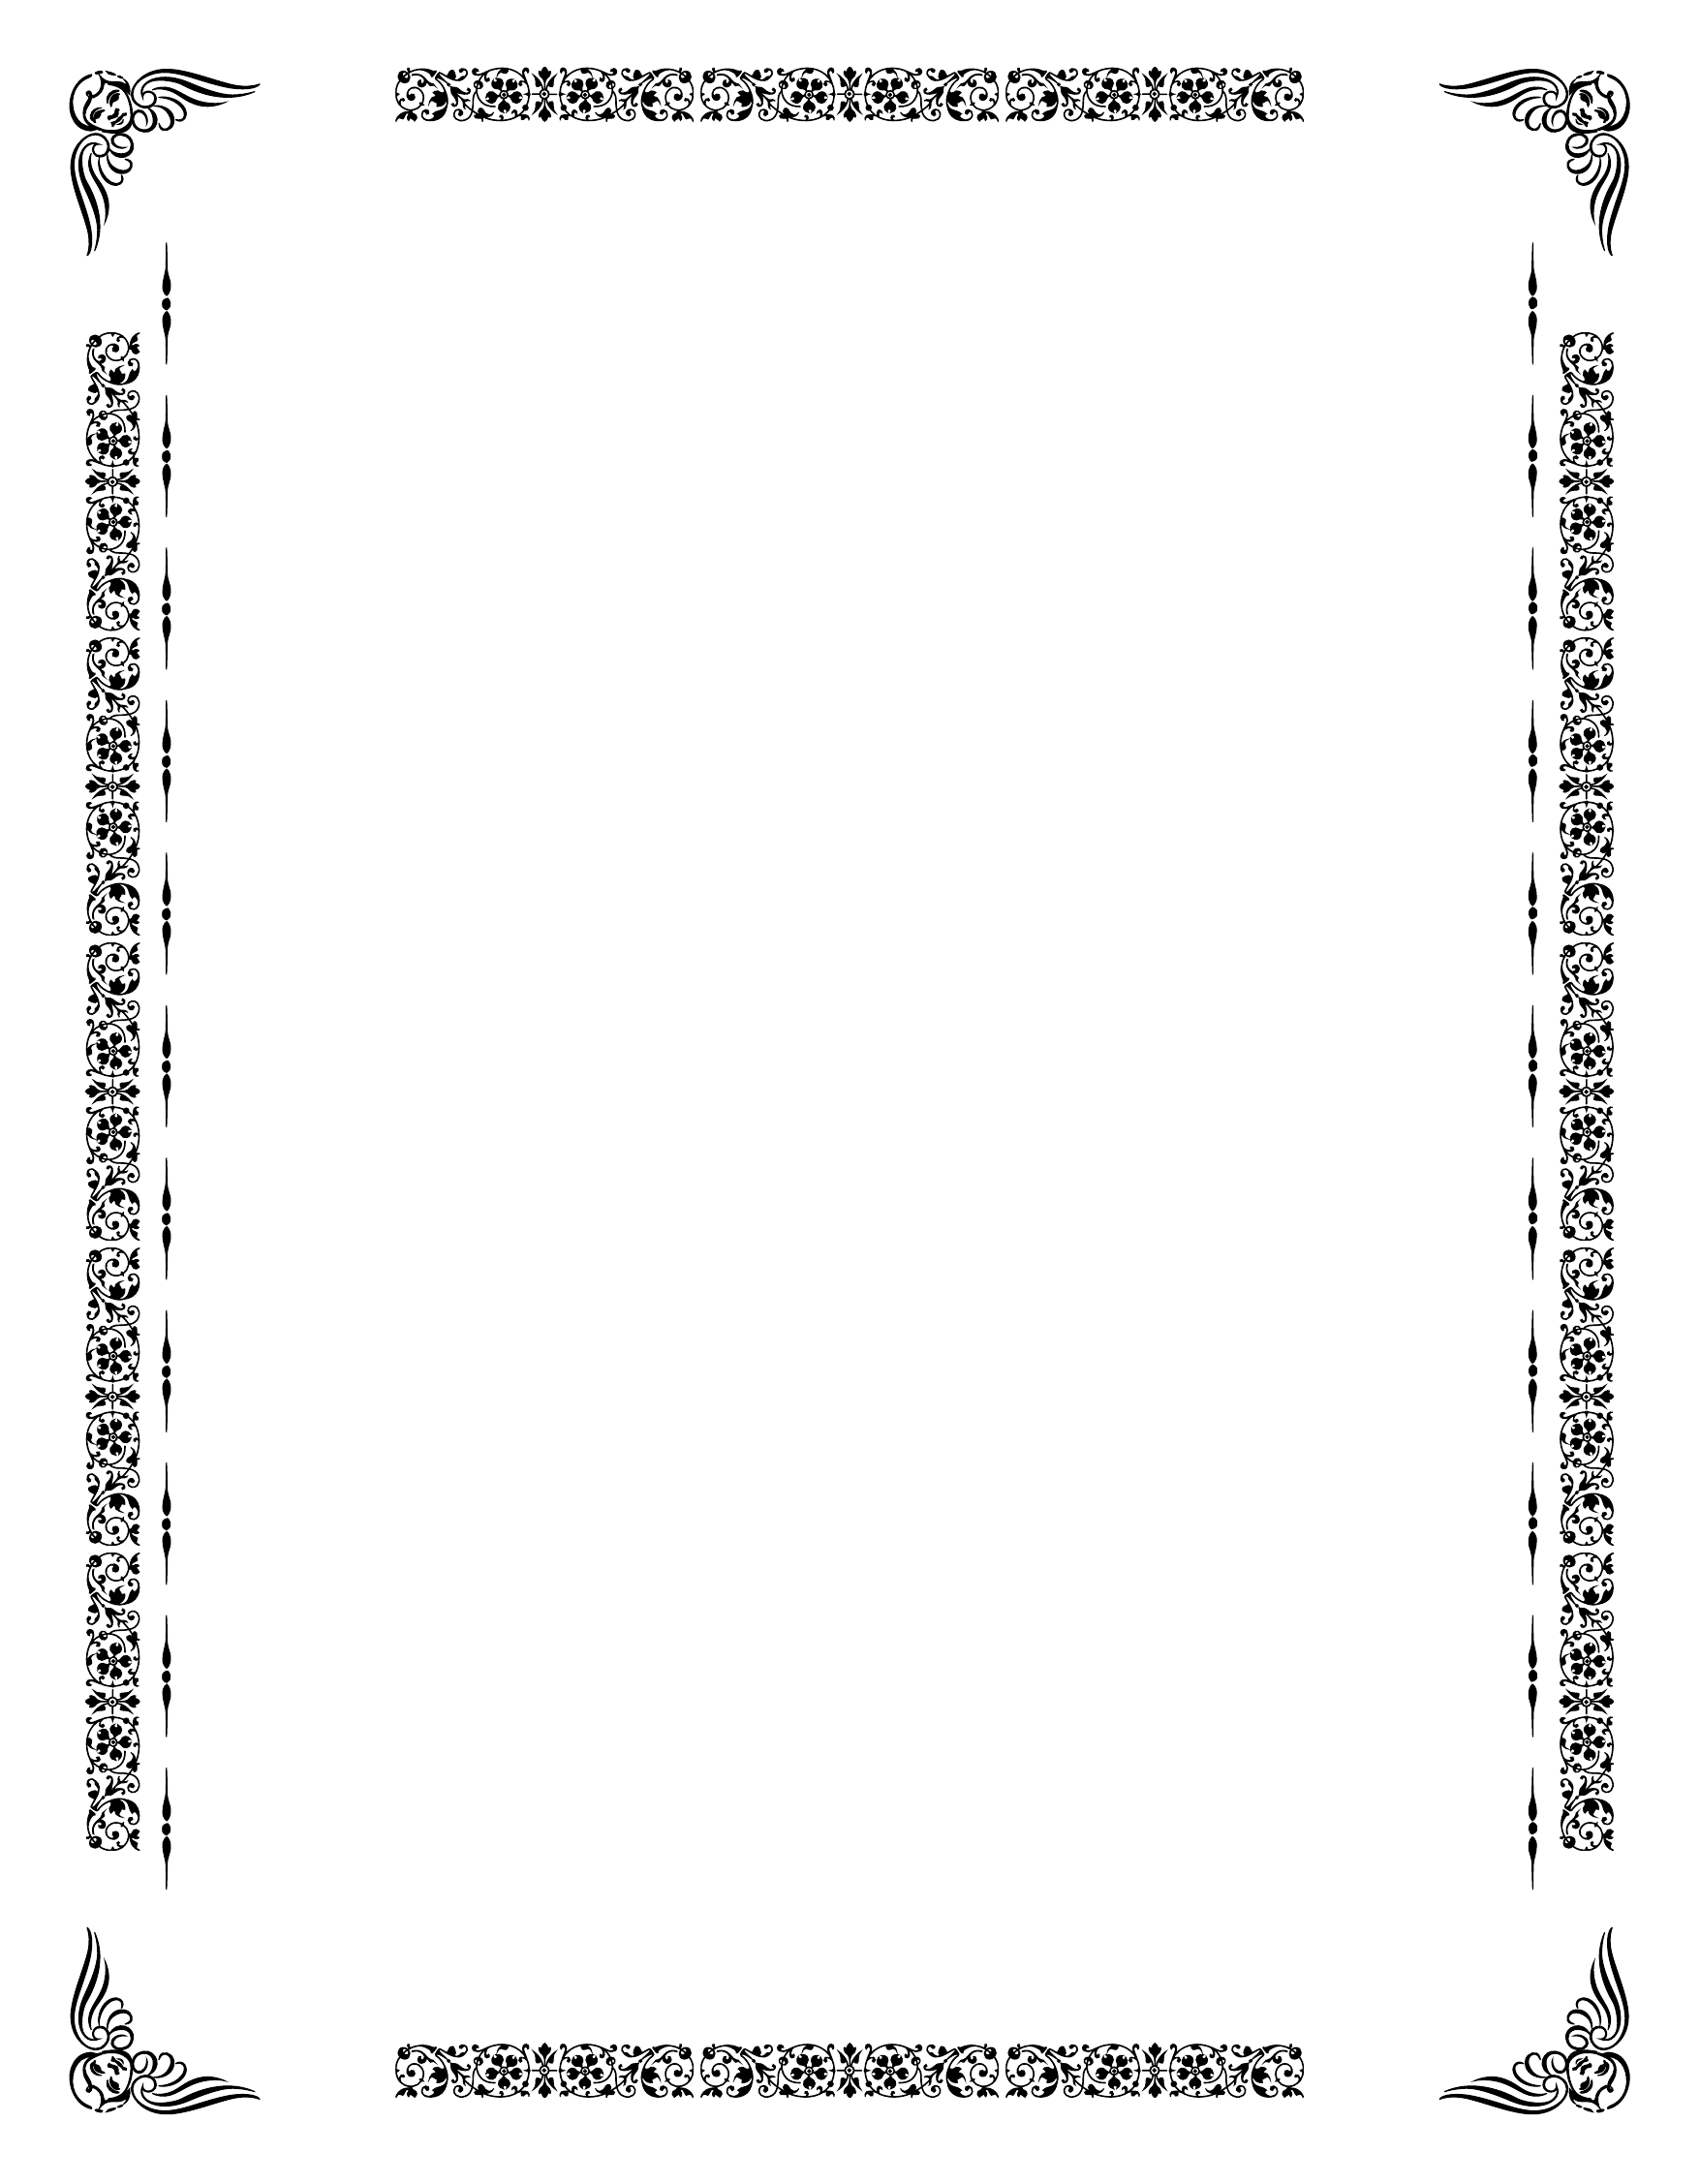
\begin{tikzpicture}[color=black, every node/.style={inner sep= 15pt}]
\node (NW) [anchor=north west] at (current page.north west){\pgfornament[width=2.5cm] {131}};
\node (NE) [anchor=north east] at (current page.north east){\pgfornament[width=2.5cm, symmetry=v]{131}};
\node (SW) [anchor=south west] at (current page.south west){\pgfornament[width=2.5cm, symmetry=h]{131}};
\node (SE) [anchor=south east] at (current page.south east){\pgfornament[width=2.5cm, symmetry=c]{131}};
\foreach \i in {-4,0,4}
\node[anchor=north,xshift=\i cm] at (current page.north){\pgfornament[scale=0.25,symmetry=v]{71}};
\foreach \i in {-4,0,4}
\node[xshift=\i cm, yshift=32.25 pt] at (current page.south){\pgfornament[scale=0.25,symmetry=v]{71}};
\foreach \i in {-8,-4,0,4,8}
\node[yshift=\i cm, xshift=32.25pt, rotate=90] at (current page.west){\pgfornament[scale=0.25,symmetry=v]{71}};
\foreach \i in {-8,-4,0,4,8}
\node[yshift=\i cm, xshift=-32.25pt, rotate=90] at (current page.east){\pgfornament[scale=0.25,symmetry=v]{71}};
\foreach \i in {-11,-9,...,7,9}
\node[anchor=west, yshift=\i cm, xshift=52.25pt, rotate=90] at (current page.west){\pgfornament[scale=0.1]{80}};
\foreach \i in {-11,-9,...,7,9}
\node[anchor=east, yshift=\i cm, xshift=-52.25pt, rotate=-90] at (current page.east){\pgfornament[scale=0.1]{80}};
\end{tikzpicture}
}}

%%%%%%%%%%%%%%%%%%%%%%%%%%%%%%%%%%%%%%%%%%%%%%%%%%%%%%%%%%%%%%%%%%%%%%%%%%%%%%%%%%%%%%%%%%%%%%%%%%%%%%%%%%%%%%%%%%

\centering % Centre everything on the title page
		
\scshape % Use small caps for all text on the title page

\vspace*{\baselineskip} % White space at the top of the page

%------------------------------------------------
%	Title
%------------------------------------------------

\rule{\textwidth}{1.6pt}\vspace*{-\baselineskip}\vspace*{2pt} % Thick horizontal rule
\rule{\textwidth}{0.4pt} % Thin horizontal rule

\vspace{0.75\baselineskip} % Whitespace above the title

{\huge \calligra{\textbf{Note for Homological Algebra} }\\} % Title

\vspace{0.75\baselineskip} % Whitespace below the title

\rule{\textwidth}{0.4pt}\vspace*{-\baselineskip}\vspace{3.2pt} % Thin horizontal rule
\rule{\textwidth}{1.6pt} % Thick horizontal rule

\vspace{2\baselineskip} % Whitespace after the title block

%------------------------------------------------
%	Subtitle
%------------------------------------------------

\Huge{范畴论笔记} 

\vspace*{3\baselineskip} % Whitespace under the subtitle



\vspace{0.5\baselineskip} 

{\scshape   \LARGE Edited by\\  颜成子游/南郭子綦} % Editor list
\vspace{0.2\baselineskip} 


\vfill 
\Large{最后一次编译时间:\DTMnow}
%------------------------------------------------
% Author
%------------------------------------------------

\begin{figure}[!h]
    \centering
    
\includegraphics[width = 3cm, height= 3cm]{resource/icon.png}%% include the university icon here
\end{figure}
\vspace{0.3\baselineskip} 

\end{titlepage}
\backgroundsetup{contents={}} %% to remove background and watermark from other pages
\tableofcontents

\quad

这是笔者于2023年本科四年级上学期学习Weibel同调代数导论的学习笔记。
\chapter{流形上的非退化光滑函数}
\section{Morse函数}
我们先用一个引理说明在非临界点$M$的平凡性质。
\begin{lemma}[非临界点]
	设$M^a=\{p\in M|f(p)\leq a\}$。若$a$不是临界值,则$M^a$是带边的光滑流形。
\end{lemma}

引理的证明留作练习。主要使用到隐函数定理以及带边流形的定义。

\begin{definition}[非退化点]
	考虑$M$上的函数$f$.若在$f$的临界点$p$处存在一个局部坐标$(U;x^i)$使得矩阵:
	\begin{align}\label{Hess}
		(\frac{\partial^2 f}{\partial x^i\partial x^j}(p))
	\end{align}
	非奇异,则称$p$是一个非退化点。
\end{definition}
这里需要注意的是,$p$的非退化性显然与局部坐标$x^i$无关。因此$p$的非退化性是$f$内蕴的性质。

如果$p$是$f$的临界点,我们就可以定义在$T_pM$上的双线性函数$f_{**}$。若$v,w \in T_pM$,用$\tilde{v}$和$\tilde{w}$表示在$p$处值为$v,w$的向量场。定义:
\begin{align}
	f_{**}(v,w)=\tilde{v}_p(\tilde{w}f)
\end{align}

我们断言:
\begin{lemma}
	$f_**$是对称的良定双线性函数。
\end{lemma}
\begin{proof}
	考虑:
	\begin{align}
		\tilde{v}_p(\tilde{w}f)-\tilde{w}_p(\tilde{v}f)=[\tilde{v},\tilde{w}]_p(f)=0
	\end{align}
	最后一个等号成立,是因为$p$是$f$的临界点。

	从而$f_{**}$是对称的。因此,$\tilde{v}_p(\tilde{w}f)$与$\tilde{v}$的选取无关,$\tilde{w}_p(\tilde{v}f)$与$\tilde{w}$的选取无关.

	于是$f_{**}$与$\tilde{v},\tilde{w}$的选取都无关,因而是良定的双线性函数。
\end{proof}
\begin{definition}[Hessian,指数,零化度]
    \quad \quad 称$f_{**}$为函数$f$在$p$处的Hessian双线性函数。
	
	而$f_{**}$的指数定义为满足$f_**$限制在上为负定双线性函数的子空间$V$的最大维数。$f_{**}$的零化度定义为$f_{**}$的零空间$W$的维数,即子空间$W=\{v \in V|f_{**}(v,w)=0,\forall w\in V\}$的维数。
\end{definition}

可以验算$f_{**}$在坐标$(U;x^i)$下给出的就是矩阵\ref{Hess}.显然,$f$在$p$处非退化等价于$f_{**}$的零化度是$0$。$f_{**}$的指数也称为$f$在$p$处的指数。

\begin{lemma}[Morse引理]\label{Morse-lemma}
	设$p$是$f$的非退化点,则存在一个$p$处的局部坐标$(U;y^i)$满足$y^i(p)=0,\forall i$且:
	\begin{align}
		f(q)=f(p)-(y^1)^2-\dots-(y^\lambda)^2+(y^{\lambda+1})^2+\dots+(y^n)^2
	\end{align}
	在整个$U$上都成立.其中$\lambda$是$f$在$p$处的指数。
\end{lemma}
\begin{proof}
	我们首先说明如果$f$拥有这样的表达式,则指数为$\lambda$.

	对于坐标$(z^i)$,若:
	\begin{align*}
		f(q)=f(p)-(z^1(q))^2-\dots-(z^\lambda(q))^2+\dots+(z^n(q))^2
	\end{align*}
	则容易求出$f_{**}$在该坐标下的矩阵为$\mathrm{diag}(-2,\dots,-2,2,\dots,2)$.其中$-2$一共有$\lambda$个。

	因此存在一个$\lambda$维的子空间使得$f_{**}$是负定的,存在一个$n-\lambda$维的子空间$V$使得$f_{**}$是正定的。如果$p$处的指数大于$\lambda$,则对应的子空间与$V$相交不为空。但这是不可能的,因此$\lambda$是$f$在$p$处的指数。

	接下来我们说明$(y^i)$坐标存在。不妨设$p$是$\R^n$的原点且$f(p)=f(0)=0$.从而有:
	\begin{align}
		f(x_1,\dots,x_n)=\int_0^1\frac{\dd f(tx_1,\dots,x_n)}{\dd   t}\dd t=\int_0^1 \sum_{i=1}^n \pa{f}{x_i}(tx_1,\dots,tx_n)x_i\dd t
	\end{align}
	令$g_j=\int_0^1\pa{f}{x_i}(tx_1,\dots,tx_n)\dd t$,则$f=\sum_j  x_jg_j$在$0$处的一个邻域上成立。

	因为$0$是$f$的临界点,从而$\pa{f}{x)i}(0)=0$。这意味着$g_j(0)=\pa{f}{x_i}(0)$.因而对$g_j$作上述$f$同样的分解:
	\begin{align*}
		f(x_1,\dots,x_n)=\sum_{i,j} x_ix_jh_{ij}(x_1,\dots,x_n)
	\end{align*}
	
	不妨假设$h_{ij}$关于$i,j$对称。通过计算,不难验证矩阵$(h_{ij}(0))$等于:
	\begin{align*}
		(\frac{1}{2}\frac{\partial^2f}{\partial x^i\partial x^j}(0))
	\end{align*}
	因此$h_{ij}(0)$是非奇异的矩阵。仿照模仿有理标准型的构造,可以证明存在一组坐标$(y^i)$使得$f$呈现为引理中的形式。具体的构造办法详见Milnor原书。(附录)
\end{proof}

Morse引理的好处在于我们可以用指数唯一确定$f$在$p$处的一个标准形式。根据这个引理,可以得知$f$在非退化点$p$的一个邻域内只有$p$一个临界点。
\begin{corollary}
	非退化临界点是离散的。特别的,紧致流形$M$上的非退化临界点只有有限个。
\end{corollary}

\begin{definition}[Morse函数]
	若$f\in \mathcal{O}(M)$且只有非退化的临界点,则称该函数为Morse函数。
\end{definition}
Morse函数的好处是显而易见的。然而存在性则是一个问题。本节我们剩下的内容为下面的定理。
\begin{theorem}
	任何流形$M$上都存在一个可微的函数$f$,满足不存在退化临界点,且$M^a$对于任何$a \in \R$都是紧致的。
\end{theorem}

根据Whitney嵌入定理,任何流形都可以嵌入到维数足够高的欧氏空间。因而我们考虑$M$是$\R^n$的$k$维嵌入子流形(之后统称为“子流形”)。

定义$N \subset M\times \R^n$为:
\begin{align*}
	N=\{(q,v):q \in M,v\in T_q\R^n,v\perp M\}
\end{align*}
即$N$是$M$在$\R^n$中的法丛。不难验证$N$是$n$维的流形,且光滑的嵌入进$\R^{2n}$中。定义$E:N \to \R^n$为映射$(q,v)\mapsto q+v$.

\begin{definition}[焦点]
	称$e \in \R^n$是$(M,q)$重数为$\mu$的焦点,若$e=E(q,v),(q,v)\in N$且$E$在$(q,v)$处的Jacobian矩阵有零化度$\mu$.
\end{definition}

根据Sard定理,两个微分流形之间的可微映射的临界点是很有限的——临界值只有$0$测度。显然焦点是$E$的临界值,因而:
\begin{corollary}\label{0focus}
	对于几乎所有的$x \in \R^n$,$x$都不是$M$的焦点。
\end{corollary}

现在固定$p \in \R^n$.定义函数$f:M \to \R$为:
\begin{align}
	L_p=f:q\mapsto\|q-p\|^2
\end{align}
在坐标$(U;u^1,\dots,u^k)$下,$f$的表达式为:
\begin{align*}
	f(u^1,\dots,u^k)=\|\vec{x}(u^1,\dots,x^k)-\vec{p}\|^2=\vec{x}\vec{x}-2\vec{x}\vec{p}+\vec{p}\vec{p}
\end{align*}

因此可以计算:
\begin{align*}
	\pa{f}{u^i}=2\pa{\vec{x}}{u^i}\cdot(\vec{x}-\vec{p})
\end{align*}

因此$q$是$f$的临界点,当且仅当$q-p$垂直与$M$垂直。

考虑$f$的二阶导数。我们有:
\begin{align*}
	\frac{\partial^2 f}{\partial u^i\partial u^j}=2\pa{\vec{x}}{u^i}\pa{\vec{x}}{u^j}+\pa{\vec{x}}{u^i}u^j\cdot(\vec{x}-\vec{p})
\end{align*}

从而有
\begin{lemma}
	$q$是$f=L_p$的退化临界点等价于$p$是$(M,q)$的焦点。根据推论\ref{0focus},总存在这样的$L_p$使得该函数不存在退化的临界点。另外,若$q$是$L_p$的退化临界点,则该点的零化度是$p$的重数。
\end{lemma}

\section{临界值处的伦形}
\section{Morse不等式}


\chapter{Morse理论的应用——测地线变分}
\section{道路的能量积分}
\section{指标定理}
\section{道路空间的伦型}

\ifx\allfiles\undefined

	% 如果有这一部分另外的package,在这里加上
	% 没有的话不需要
	\newcommand{\id}{\mathrm{id}}
\newcommand{\Hom}{\mathrm{Hom}}
\newcommand{\N}{\mathbb{N}}
\newcommand{\Z}{\mathbb{Z}}
\newcommand{\Q}{\mathbb{Q}}
\newcommand{\R}{\mathbb{R}}
\newcommand{\C}{\mathbb{C}}
\newcommand{\HH}{\mathbb{H}}
\newcommand{\RP}{\mathbb{RP}}
	\begin{document}
\else
\fi
\chapter{Tor函子和Ext函子}
本章的目的是介绍Tor函子和Ext函子的诸多性质。他们是同调代数初等应用中的常客。
\section{Abel群的Tor函子}
我们首先观察一个经典的PID上的模——Abel群的Tor函子。其实,Tor函子的名字就来源于其对Abel群的研究。

\begin{example}{}
    对于Abel群$B$而言,$\mathrm{Tor}_0^{\Z}(\Z/p,B)=B/pB$,$\mathrm{Tor}_1^\Z(\Z/p,B)={}_pB=\{b \in B:pB=0\}$.对于$n\geq 2$,$\mathrm{Tor}_2^\Z(\Z/p,B)=0$.

    上述结果可以这么看。取$\Z/p$的投射解消
    \begin{align}
        0 \to \Z \stackrel{p}{\rightarrow}\Z \to \Z/p \to 0
    \end{align}
    从而我们计算的是:
    \begin{align}
        0 \to B \stackrel{p}{\rightarrow} B \to 0
    \end{align}
    的同调群。
\end{example}
 特殊情况下,Tor函子表现出$1$阶挠子群,高阶为$0$的特点。实际上,我们有下面的命题:
 \begin{proposition}{}
    对于两个Abel群$A$,$B$,我们有:
    
    (a)$\mathrm{Tor}_1^\Z(A,B)$是一个挠群。

    (b)$\mathrm{Tor}_n^\Z(A,B)$在$n \geq 2$的情况下为$0$.
 \end{proposition}
 \begin{proof}
    证明依赖Tor函子与滤过余极限交换性。$A$是其有限生成子群的滤过余极限,所以$\mathrm{Tor}_n(A,B)$是$\mathrm{Tor}_n(A_\alpha,B)$的滤过余极限。

    Abel群的余极限总是他们直和的商子群。所以我们只需要证明对于有限生成子群上述命题成立即可。

    设$A=\Z^m \oplus \Z/p_1 \oplus \Z/p_2 \dots \Z/p_r$。因为$\Z^m$是投射的,所以只用考虑:
    \begin{align}
        \mathrm{Tor}_n(A,B)=\mathrm{Tor}_n(\Z/p_1,B)\oplus \mathrm{Tor}_n(\Z/p_2,B) \oplus \dots \mathrm{Tor}_n(\Z_r,B)
    \end{align}
    于是根据之前的例子我们知道结论成立。
 \end{proof}
 \begin{proposition}{}
    $\mathrm{Tor}_1^\Z(\Q/\Z,B)$是$B$的挠子群。
 \end{proposition}
 \begin{proof}
    可以想见,$\Z/p$提取出$B$中挠性为$p$的元素。$\Q/\Z$是其有限子群的滤过极限,并且每个有限子群都同构于某个$\Z/p$($p$不一定是素数。)
    \begin{align}
        \mathrm{Tor}_*^\Z(\Q/\Z,B)\cong \Colim \mathrm{Tor}_1^\Z(\Z/p,B)\cong \Colim({}_pB)=\cup_p\{b\in B:pb=0\}
    \end{align}

 \end{proof}
 \begin{proposition}{}
    如果$A$是一个无挠交换群,则$\mathrm{Tor}_n(A,B)$对于$n \neq 0$和Abel群$B$总是$0$。
 \end{proposition}
 \begin{proof}
    $A$是有限生成子群的滤过余极限。然而$A$无挠意味着这些有限生成子群都是自由群。用Tor保滤过余极限即可。
 \end{proof}
 如果$R$是交换环,则张量积有典范的同构,因此$\mathrm{Tor}_*(A,B)\cong \mathrm{Tor}_*(B,A)$.

 \begin{corollary}{}
    $\mathrm{Tor}_1^\Z(A,-)=0$等价于$A$无挠等价于$\mathrm{Tor}_1^\Z(-,A)=0$.
 \end{corollary}
 但是Tor函子并非对于所有环都有这么好的性质。比如下面的例子就说明在$R=\Z/m$的情况下可能失败:
 \begin{example}{}
   设$R=\Z/m$,$A=\Z/d$。其中$d|m$。从而$A$是$R$模。

   我们考虑$A$周期性的自由解消:
   \begin{align}
      \dots \to \Z/m \to Z/m \to \Z/m \to \Z/d
   \end{align}
   其中从$\Z/m$到$\Z/d$的映射是商映射,而$\Z/m$各自之间交替出现$d$和$m/d$。所以对于任何一个$\Z/m$模$B$,我们都有:
   \begin{align}
      \mathrm{Tor}_n^{\Z/m}(\Z/d,B)=\begin{cases}
      B/dB,n=0\\ \{b\in B:db=0\}/(m/d)B,n \text{是奇数}\\ \{b \in B:(m/d)b=0\}/dB,n \text{是偶数且}>0
      \end{cases}
   \end{align}
 \end{example}
 然而我们可以尝试对下面特殊的情况进行一些讨论。
 \begin{example}{}
   设$r$是$R$的一个左非零除子。即${}_rR=\{s \in R|rs=0\}$是$0$。对于每个$R$模$B$,记${}_rB=\{b \in B:rb=0\}$。用$R/rR$代替上述$\Z/p\Z$,用相同的计算办法可以算的:
   \begin{align}
      \mathrm{Tor}_0(R/rR,B)=B/rB;\quad \mathrm{Tor}_1^R(R/rR,B)={}_r B; \quad \mathrm{Tor}_n^R(R/rR,B)=0, n\geq 0
   \end{align}
 \end{example}
 \begin{proposition}{}
   若${}_r R\neq 0$,我们只能得到一个并非投射的解消:
   \begin{align}
      0 \to {}_r R \to R \stackrel{r}{\rightarrow} R \to R/rR \to 0
   \end{align}
   然而第二章我们介绍了dimension shelfting办法\ref{dim-Shifting}。所以我们对于$n \geq 3$,存在:
   \begin{align}
      \mathrm{Tor}_n^R(R/rR,B) \cong \mathrm{Tor}_{n-2}^R({}_r R,B)
   \end{align}

   其次,还有正合列:
   \begin{align}
      0 \to \mathrm{Tor}_2^R(R/rR,B) \to {}_rR \otimes B \to {}_rB \to \mathrm{Tor}_1^R(R/rR,B) \to 0
   \end{align}
   因为$\mathrm{Tor}_2^R(R/rR,B)$是$0 \to {}_rR\otimes B \to R\otimes B=B$的核。而该映射的像就在${}_r B$中,所以上述正合列中第一个和第二个已经确实成立。

   考虑$\mathrm{Tor}_1(R/rR,B)$。根据导引长正合列:
   \begin{align}
      0 \to \mathrm{Tor}_1(R/rR,B) \to rR\otimes B \to B \to B/rB
   \end{align}
   为了定义${}_r B \to \mathrm{Tor}_1(R/rR,B)$.我们定义${}_r B \to rR\otimes B$.即$b \mapsto r \otimes b$。则该映射实际上打进$\mathrm{Tor}_1(R/rR,B)$.

   若$\sum (rr_i)\otimes b_i \in \mathrm{Tor}_1(R/rR,B)$且在$B$中像为$\sum r(1\otimes r_ib_i)=0$,则${}_r B$中$\sum r_ib_i$的像是$\sum (rr_i)\otimes b_i$。于是我们定义了满射。

   最后需要说明${}_r B$处的正合。若$r \otimes b=0$,则存在$r_i$和$b_i$使得$rr_i=0$,$b=\sum r_ib_i$.
 \end{proposition}
 \begin{proposition}{}
   设$R$是交换整环,分式域$F$。则$\mathrm{Tor}_1^R(F/R,B)$是$B$的挠子群:$\{b \in B:(\exists r\neq 0)rb=0\}$
 \end{proposition}
 \begin{proposition}{}
   $\mathrm{Tor}_1^R(R/I,R/J) \cong \dfrac{I\cap J}{IJ}$对于任何右理想$I$和左理想$J$都成立。特别的,对于双边理想$I$:
   \begin{align}
      \mathrm{Tor}_1(R/I,R/I)\cong I/I^2
   \end{align}
 \end{proposition}
 \begin{proof}
   % https://q.uiver.app/#q=WzAsMTYsWzAsMSwiMCJdLFsxLDEsIklKIl0sWzIsMSwiSSJdLFszLDEsIklcXG90aW1lcyBSL0oiXSxbNCwxLCIwIl0sWzEsMiwiSiJdLFsyLDIsIlIiXSxbMywyLCJSXFxvdGltZXMgUi9KIl0sWzAsMiwiMCJdLFs0LDIsIjAiXSxbMSwwLCIwIl0sWzEsMywiSi8oSUopIl0sWzIsMCwiMCJdLFsyLDMsIlIvSSJdLFszLDAsIlxca2VyIGkiXSxbMywzLCJSL0kgXFxvdGltZXMgUi9KIl0sWzAsMV0sWzEsMl0sWzIsM10sWzMsNF0sWzEsNV0sWzIsNl0sWzMsNywiaVxcb3RpbWVzXFxtYXRocm17aWR9Il0sWzgsNV0sWzUsNl0sWzYsN10sWzcsOV0sWzEwLDFdLFs1LDExXSxbMTIsMl0sWzYsMTNdLFsxNCwzXSxbNywxNV0sWzEwLDEyXSxbMTIsMTRdLFsxNCwxMSwiIiwxLHsic3R5bGUiOnsiYm9keSI6eyJuYW1lIjoiZGFzaGVkIn19fV0sWzExLDEzXSxbMTMsMTVdXQ==
\[\begin{tikzcd}
	& 0 & 0 & {\ker i} \\
	0 & IJ & I & {I\otimes R/J} & 0 \\
	0 & J & R & {R\otimes R/J} & 0 \\
	& {J/(IJ)} & {R/I} & {R/I \otimes R/J}
	\arrow[from=2-1, to=2-2]
	\arrow[from=2-2, to=2-3]
	\arrow[from=2-3, to=2-4]
	\arrow[from=2-4, to=2-5]
	\arrow[from=2-2, to=3-2]
	\arrow[from=2-3, to=3-3]
	\arrow["{i\otimes\mathrm{id}}", from=2-4, to=3-4]
	\arrow[from=3-1, to=3-2]
	\arrow[from=3-2, to=3-3]
	\arrow[from=3-3, to=3-4]
	\arrow[from=3-4, to=3-5]
	\arrow[from=1-2, to=2-2]
	\arrow[from=3-2, to=4-2]
	\arrow[from=1-3, to=2-3]
	\arrow[from=3-3, to=4-3]
	\arrow[from=1-4, to=2-4]
	\arrow[from=3-4, to=4-4]
	\arrow[from=1-2, to=1-3]
	\arrow[from=1-3, to=1-4]
	\arrow[dashed, from=1-4, to=4-2]
	\arrow[from=4-2, to=4-3]
	\arrow[from=4-3, to=4-4]
\end{tikzcd}\]
上图是蛇形引理\ref{snake}.验证$I/(IJ)$和$I \otimes R/J$有典范同构可以得出第一行正合。第二行则典范正合。

 最右边的列是计算$\mathrm{Tor}_1(R/I,R/J)$的定义式。感觉Dimesion Shifting,$\ker i$是$\mathrm{Tor}_1(R/I,R/J)$。根据snake引理,$\ker i$是$J/(IJ)  \to R/I$的核:$\dfrac{I\cap J}{IJ}$。
 \end{proof}
\section{Tor函子与平坦性}
我们在这一节着重研究Tor函子的ayclic对象——平坦对象。
\begin{definition}[平坦模]{flat-module}
   称一个左$R$模是平坦模,若函子$\otimes_R B$是正合函子。同样,对于右$R$模,也可以定义类似的平坦性。
\end{definition}
如果$A$是投射的,则$\mathrm{Tor}_n(A,B)=0$。不难说明$A$此时是平坦的。因为投射模一定是平坦模。然而平坦模不一定是投射模。例如$\Q$作为交换群而言是平坦的,但不是投射的。(为什么?)
\begin{theorem}{}
   若$S$是$R$中的乘法封闭集,则$S^{-1}R$是一个平坦模。
\end{theorem}
这个定理当然很交换代数,不过影响不大,我们可以尝试证明:
\begin{proof}
   构造一个滤过范畴$I$。对象是$S$中的元素,态射$\Hom_I(s_1,s_2)=\{s \in S:s_1s=s_2\}$。定义函子$F:I \to R$。$F(s)=R$,$F(s_1 \to s_2)$则定义为$R$上该态射自然给出的右乘法。

  
我们断言$F$的余极限$\Colim F(s) \cong S^{-1}R$。从而因为$S^{-1}R$是平坦模的滤过余极限,所以其是平坦的。

   下面计算$\Colim F$。首先定义$F(s) \to S^{-1}R$的映射为$r \mapsto r/s$.这样交换图显然成立:
   % https://q.uiver.app/#q=WzAsMyxbMCwwLCJGKHNfMSk9UjpyIl0sWzEsMCwiRihzXzIpPVI6cnMiXSxbMCwxLCJTXnstMX1SOnIvc18xPXJzLyhzXzFzKT1ycy9zXzIiXSxbMCwxLCJzIl0sWzAsMl0sWzEsMl1d
\[\begin{tikzcd}
	{F(s_1)=R:r} & {F(s_2)=R:rs} \\
	{S^{-1}R:r/s_1=rs/(s_1s)=rs/s_2}
	\arrow["s", from=1-1, to=1-2]
	\arrow[from=1-1, to=2-1]
	\arrow[from=1-2, to=2-1]
\end{tikzcd}\]

如果存在一个新的$B$使得余极限中关系成立,我们直接定义$S^{-1}R$中的元素$r/s$到$B$的态射为$F(s)=R$中$r$在$B$中的像即可。这是唯一的定义方式!
\end{proof}
\begin{proposition}[Tor和平坦]
   下面三个命题等价:

   (1)$B$是平坦模。

   (2)$\mathrm{Tor}_n^R(A,B)=0,\forall n\neq 0$

   (3)$\mathrm{Tor}_1^R(A,B)=0$
\end{proposition}
\begin{corollary}
   若$0 \to A \to B \to C \to 0$是正合列且$B,C$是平坦模,则$A$平坦。
\end{corollary}
\begin{proposition}
   设$R$是主理想整环,则$B$平坦等价于$B$无挠。
\end{proposition}
对于上述命题,我们给出一个反例。首先平坦显然无挠。但是无挠不一定平坦。设$k$是域且$R=k[x,y]$。$R$是经典的非主理想整环。设$I=(x,y)R$。考虑$k=R/I$有投射解消:
\begin{align}
   0 \to R \to R^2 \to R \to k
\end{align}
其中第一个$R$到$R^2$为$[-y,x]$.而$R^2$到$R$为$(x,y)$.从而$\mathrm{Tor}_1^R(I,k)\cong \mathrm{Tor}_2^R(k,k)\cong k$。于是$I$不是平坦模。

我们深入的研究一下平坦模。
\begin{definition}[Pontrjagin对偶]{Pontrjagi}
   左模$B$的Pontrjagin对偶模$B^*$是一个右模:
   \begin{align}
      B^*:=\Hom_{\mathrm{Ab}}(B,\Q/\Z); (fr)(b)=f(rb)
   \end{align}
\end{definition}
\begin{proposition}{}
   下面的命题等价。

   (1)$B$平坦。

   (2)$B^*$内射。

   (3)$I\otimes_R B\cong IB=\{x_1b_1+\dots+x_nb_n\in B:x_i\in I,b_i\in B\}$对于任何右理想$I$都成立。

   (4)$\mathrm{Tor}_I^R(R/I,B)=0$对于任何右理想$I$都成立。
\end{proposition}
\begin{proof}
   (3)和(4)的等价性来源于正合列:
   \begin{align}
      0 \to \mathrm{Tor}_1(R/I,B) \to I\otimes B \to B \to B/IB \to 0
   \end{align}
   现在考虑$A'$是$A$的子模。考虑:
   \begin{align}
      \Hom(A,B^*) \to \Hom(A',B^*)
   \end{align}
   $B^*$等价于说上述映射是满射。根据伴随关系,我们有:
   \begin{align}
      \Hom(A\otimes B,\Q/\Z) \to \Hom(A'\otimes B,\Q/Z)
   \end{align}是满射。即$(A\otimes B)^* \to (A'\otimes B)^*$是满射。

   用下面的\textbf{引理},可以知道此时$A' \otimes B \to A\otimes B$是单射,所以$B$是平坦模。同理也可以反推回去。所以(1)(2)等价。另外带入$A'=I,A=R$,可以推出$I\otimes B \to R\otimes B$是单射。于是$I\otimes B\cong IB$且根据Baer判别法,这是可逆的。所以(1)(3)等价。
\end{proof}
我们描述一个引理。
\begin{lemma}{}
   $f:A' \to A$是单射等价于$f^*:A^* \to A'^*$是满射。
\end{lemma}
\begin{proof}
   因为$\Q/\Z$是内射的$\Z$模,所以保正合。
\end{proof}
\begin{proposition}[Pontrjagin对偶与正合]{}
   $A \to B \to C$是正合的当且仅当对偶$C^* \to B^* \to A^*$是正合的。
\end{proposition}
\begin{proof}
   因为$\Q/\Z$是内射模,所以$\Hom(-,\Q/\Z)$是正合函子,因此$C^* \to B^* \to A^*$是正合的。

   如果$C^* \to B^* \to A^*$正合,则$A \to B \to C$首先复形。若$b \in B$且在$C$中的像为$0$,我们证明$b$在$A$的像中。若不然,则$b+\mathrm{im}A$是$B/\mathrm{im}A$中的非$0$元。我们定义$g:B/\mathrm{im}A \to \Q/\Z$使得$g(b+\mathrm{im}A)\neq 0$。则$g$也给出了$B^*$中的非$0$元且在$A^*$中的像为$0$。

   所以可以给出一个$f \in C^*$。剩下的就是显然了。
\end{proof}
这个证明写的比较模糊。

我们邀请读者回忆有限展示的概念。然后不加证明的给出有限展示与生成元的选取无关.

\begin{proposition}{}
   若$\varphi:F \to M$是满射且$F$是有限生成的,$M$是有限展示的,则$\ker \varphi$是有限生成的。
\end{proposition}
HINT:用蛇形引理。

仍然用$A^*$表示$A$的Pontrjagin对偶,则存在一个自然的映射$\sigma:A^* \otimes_R M \to \Hom_R(M,A)^*$
\begin{align}
   \sigma(f\otimes m)=h \mapsto f(h(m))
\end{align}
其中$f\in A^*,m \in M,h \in \Hom(M,A)$.我们的问题是,什么时候$\sigma$是一个同构?
\begin{theorem}{}
   对于任何有限展示的$M$,$\sigma$都是一个同构。
\end{theorem}
\begin{proof}
   若$M=R$,则自然有$\sigma$是同构。根据可加性,$M=\R^n$的时候也是如此。所以有:
   % https://q.uiver.app/#q=WzAsOCxbMCwwLCJBXipcXG90aW1lcyBSXm0iXSxbMCwxLCJcXEhvbShSXm0sQSleKiJdLFsxLDAsIkFeKlxcb3RpbWVzIFJebiJdLFsyLDAsIkFeKlxcb3RpbWVzIE0iXSxbMywwLCIwIl0sWzMsMSwiMCJdLFsyLDEsIlxcSG9tKE0sQSleKiJdLFsxLDEsIlxcSG9tKFJebixBKV4qIl0sWzAsMV0sWzAsMl0sWzIsM10sWzMsNF0sWzYsNV0sWzcsNl0sWzEsN10sWzIsN10sWzMsNl1d
\[\begin{tikzcd}
	{A^*\otimes R^m} & {A^*\otimes R^n} & {A^*\otimes M} & 0 \\
	{\Hom(R^m,A)^*} & {\Hom(R^n,A)^*} & {\Hom(M,A)^*} & 0
	\arrow[from=1-1, to=2-1]
	\arrow[from=1-1, to=1-2]
	\arrow[from=1-2, to=1-3]
	\arrow[from=1-3, to=1-4]
	\arrow[from=2-3, to=2-4]
	\arrow[from=2-2, to=2-3]
	\arrow[from=2-1, to=2-2]
	\arrow[from=1-2, to=2-2]
	\arrow[from=1-3, to=2-3]
\end{tikzcd}\]
    因为$\otimes$是右正合的,$\Hom$是左正合的,所以图中两个行正合.根据5引理\ref{5lemma}可知$\sigma$是同构。
\end{proof}
\begin{theorem}{}
   每个有限展示的平坦模是投射模。
\end{theorem}
\begin{proof}
   我们证明$\Hom(M,-)$是正合的。设$B\to C$是满射,则$C^* \to B^*$是单射。若$M$是平坦的,则:
   % https://q.uiver.app/#q=WzAsNCxbMCwwLCJDXipcXG90aW1lc19SIE0iXSxbMSwwLCJCXipcXG90aW1lcyBNIl0sWzAsMSwiXFxIb20oTSxDKV4qIl0sWzEsMSwiXFxIb20oTSxCKV4qIl0sWzAsMV0sWzAsMiwiXFxzaWdtYSJdLFsxLDMsIlxcc2lnbWEiLDJdLFsyLDNdXQ==
\[\begin{tikzcd}
	{C^*\otimes_R M} & {B^*\otimes M} \\
	{\Hom(M,C)^*} & {\Hom(M,B)^*}
	\arrow[from=1-1, to=1-2]
	\arrow["\sigma", from=1-1, to=2-1]
	\arrow["\sigma"', from=1-2, to=2-2]
	\arrow[from=2-1, to=2-2]
\end{tikzcd}\]
   给出了$\Hom(M,B)\to Hom(M,C)$的满射。所以$M$是投射模。
  \end{proof}  
   下面的引理来源于dimension shifting.
   \begin{lemma}[平坦解消引理]{}
      群$\mathrm{Tor}_*(A,B)$可以用平坦模进行计算。
   \end{lemma}
\begin{proposition}[Tor的平坦基变换]
    设$R \to T$是环同态,使得$T$成为了$R$模。从而对于所有的$R$模$A$,所有的$T$模$C$和所有的$n$:
    \begin{align}
      \mathrm{Tor}_n^R(A,C)\cong \mathrm{Tor}_n^T(A \otimes_R T,C)
    \end{align}
\end{proposition}
\begin{proof}
   选择$R$模的投射解消$P \to A$,则$\mathrm{Tor}_*^R(A,C)$是$P \otimes_R C$的同调。

   因为$T$是平坦的$R$模,所以$P_n\otimes T$是投射的$T$模且$P\otimes T \to A \otimes T$是$T$模的投射解消。所以$\mathrm{Tor}_n^T(A \otimes T,C)$是复形$(P\otimes_R T)\otimes_T C \cong P\otimes_R C$的同调。
\end{proof}
\begin{corollary}{}
   若$R$是交换环,$T$是平坦的$R$代数,则对于所有的$R$模$A,B$和所有的$n$:
   \begin{align}
      T\otimes_R \mathrm{Tor}_n^R(A,B)\cong \mathrm{Tor}_n^T(A\otimes_R T,T\otimes_R B)
   \end{align}
\end{corollary}
\begin{proof}
   设$C=T\otimes_R B$.根据上面的命题,我们只需要证明$\mathrm{Tor}_*^R(A,T\otimes B)=T\otimes \mathrm{Tor}_*^R(A,B)$.因为$T\otimes_R$是正合函子,所以$T\otimes \mathrm{Tor}_*^R(A,B)$是$T\otimes_R (P\otimes _R B)$的同调,从而为$\mathrm{Tor}_*^R(A,T\otimes B)$.
\end{proof}
为了使得$\mathrm{Tor}$给出模结构,我们必须假设$R$是交换环。原因是下面的引理:

\begin{lemma}{}
   设$\mu:A \to A$是左乘一个中心元$r$。则诱导的$\mu_*:\mathrm{Tor}_n^R(A,B)\to \mathrm{Tor}_n^R(A,B)$也是左乘$r$.
\end{lemma}
\begin{proof}
   选择$A$的投射解消$P \to A$。左乘$r$是一个$R$模的链复形映射$\tilde{\mu}:P \to P$.(因为$r$是一个中心元)。从而$\tilde{mu}\otimes B$是$P\otimes B$的$r$左乘。作为商群$\mathrm{Tor}$也是如此。
\end{proof}
\begin{corollary}{}
   若$A$是一个$R/r$模,则对于每个$R$模$B$,$R$模$\mathrm{Tor}_*^R(A,B)$也是$R/r$模。换句话说,$rR$乘在该模得$0$.
\end{corollary}
\begin{corollary}[Tor的局部化]{}
   若$R$是一个交换环且$A,B$都是$R$模。下面的命题对于所有$n$都成立:
   \begin{enumerate}
      \item $\mathrm{Tor}_n^R(A,B)=0$
      \item 对于$R$的任意素理想$p$,$\mathrm{Tor}_n^{R_p}(A_p,B_p)=0$
      \item 对于$R$的任意极大理想$m$,$\mathrm{Tor}_n^{R_m}(A_m,B_m)=0$.
   \end{enumerate}
\end{corollary}
\begin{proof}
   对于$R$模而言,$M=0$等价于任意素理想$p$,$M_p=0$等价于任意极大理想$m$,$M_m=0=0$.设$M=\mathrm{Tor}(A,B)$:
   \begin{align}
      M_p=R_p \otimes_R M=\mathrm{Tor}_n^{R_p}(A_p,B_p)
   \end{align}
\end{proof}
\section{性质较好的环的Ext函子}
讨论了Ext后,我们讨论Ext函子的性质。首先我们计算一些性质很好的环的Ext函子。

\begin{lemma}{}
   $\mathrm{Ext}_\Z^n(A,B)=0$,$\forall n \geq 2$和所有的交换群$A,B$.
\end{lemma}
\begin{proof}
   把$B$嵌入到一个内射的交换群$I^0$.其商群$I^1$是可除的,因而是内射的,所以我们给出了$B$的内射解消$0 \to B \to I^0 \to I^1 \to 0$.

   所以$\mathrm{Ext}^*(A,B)$可以计算为:
   \begin{align}
      0 \to \Hom(A,I^0) \to \Hom(A,I^1) \to 0
   \end{align}
   的上同调。
\end{proof}
因此我们只需要考虑$n=1$的情况。
\begin{example}{}
   $\mathrm{Ext}_{\Z}^0(\Z/p,B)={}_p B$.$\mathrm{Ext}_\Z^1(\Z/p,B)=B/pB$.

   可以使用$0 \to \Z \to \Z \to \Z/p$作为$\Z/p$的投射解消计算。
\end{example}

因为$\Z$是投射模,所以$\Ext^1(\Z,B)=0$对于任何$B$总是成立。我们可以依据这个结果和上述结果,在$A$是有限生成的Abel群时计算$\Ext(A,B)$:
\begin{align}
   A\cong \Z^m \oplus \Z/p  \Rightarrow \Ext(A,B)=\Ext(\Z/p,B)
\end{align}
然而无限生成的情况因为余极限不交换,要复杂得多。
\begin{example}[$B=\Z$]{}
   设$A$是一个挠群,用$A^*$表示Pontrjagin对偶。$\Z$有经典的内射解消:$0 \to \Z \to \Q \to \Q/\Z \to 0$。用这个解消计算$\Ext^*(A,\Z)$:
   \begin{align}
      0 \to \Hom(A,\Q) \to \Hom(A,\Q/\Z) \to 0 
   \end{align}
   从而$\Ext_\Z^0(A,\Z)=\Hom(A,\Z)=0$,$\Ext_\Z^1(A,\Z)=A^*$。

   为了对这个例子有更深的印象,注意到$\Z_{p^\infty}$是$\Z/p^n$的余极限(并).于是可以计算:
   \begin{align}
      \Ext_\Z^1(\Z_{p^\infty},\Z)=(\Z_{p^\infty})^*
   \end{align}
   这个群是$p$-adic整数的无挠群,$\hat{\Z}_p=\Lim (\Z/p^n)$。

   再考虑一个例子:$A=\Z[1/p],B=\Z$.此时:
   \begin{align}
      0 \to \Q=\Hom(\Z[1/p],\Q) \to \Hom(\Z[1/p],\Q/\Z) \to 0
   \end{align}
   $\Ext^0$比较容易,我们考虑$\Ext^1$.此时给定$f \in \Hom(\Z[1/p],\Q/\Z)$,筛出掉$\Hom(\Z[1/p],\Q)$的元素,本质上留存的是一个$p$-adic数。并且若两个$p$-adic数只差一个整数,与他们给出的$f$是一致的。因此$\Ext^1(\Z[1/p],\Z)=\Z_{p^\infty}$。

   这说明$\Ext$对于平坦模而言也不是vanish的。
\end{example}
\begin{example}[$R=\Z/m$,$B=\Z/p$]{}
   $\Z/p$在这种情况下有无穷的周期内射解消:
   \begin{align}
      0 \to \Z/p \xrightarrow{\iota} \Z/m \xrightarrow{p}  \Z/m \xrightarrow{m/p} \Z/m \xrightarrow{p} \dots 
   \end{align}

   于是$\Ext_{\Z/m}^n(A,\Z/p)$可以计算为:
   \begin{align}
      0 \to \Hom(A,\Z/m) \to \Hom(A,\Z/m) \to \Hom(A,\Z/m) \dots
   \end{align}
   的上同调。

   比如,若$p^2|m$,则$\Ext_{\Z/m}^n(\Z/p,\Z/p)=\Z/p$
\end{example}
\begin{proposition}{}
   对于所有的$n$和$R$:
   \begin{enumerate}
      \item $\Ext_R^n(\bigoplus_\alpha A,B)\cong \prod_{\alpha}\Ext_R^n(A_\alpha,B)$
      \item $\Ext_R^n(A,\prod_\beta B) \cong \prod_\beta \Ext_R^n(A,B_\beta)$
   \end{enumerate}
\end{proposition}
\begin{proof}
   设$P_\alpha$是$A_\alpha$的投射解消。于是$\oplus P_\alpha$是$\oplus A_\alpha$的投射解消。同理,$Q_\beta$是$B_\beta$的内射解消,则$\prod Q_\beta$是$\prod B_\beta$的内射解消。

   根据$\Hom$的性质,再加上:
   \begin{align}
      H^*(\prod C_\gamma)\cong \prod H^*(C_\gamma)
   \end{align}
   可得结果。
\end{proof}
\begin{lemma}{}
   设$R$是交换环,则$\Hom_R(A,B)$和$\Ext^*(A,B)$都是$R$模。若$\mu,\tau$分别是$r$的左乘($A,B$),则诱导的$\mu^*$和$\tau^*$也是左乘。
\end{lemma}
可以看到,这是Tor函子的相似版本,可用于给出Ext与局部化交换的性质。
\begin{proof}
   给$P \to A$投射解消.左乘$r$给出了$\tilde{mu}:P \to P$作为链复形映射。映射$\Hom(\tilde{mu},B)$是$\Hom(P,B)$上链复形,是左乘$r$.

   因此商群$\Ext^n(A,B)$被$\mu^*$作用也是$r$左乘。
\end{proof}
\begin{corollary}{}
   设$R$是交换环,$A$是$R/r$模。则对于$R$模$B$,$\Ext^*_R(A,B)$是$R/r$模。
\end{corollary}
接下来的引理,定理我们不写证明,读者可自查Weibel原书。

考虑$S^{-1}\Hom_R(A,B)$.其到$\Hom_{S^{-1}R}(S^{-1}A,S^{-1}B)$有一个自然的态射$\Phi$。但这个态射一般不是同构。
\begin{lemma}{}
   如果$A$是有限展示的$R$模,则对于每个中心可乘集合$S$,$\Phi$是同构。
\end{lemma}
不难想象证明用到的是5引理\ref{5lemma}。

\begin{proposition}{}
   设$A$是交换Noether环上的有限生成模.则$\Phi$也诱导了Ext的同构:
   \begin{align}
      \Phi:S^{-1}\Ext_R^n(A,B) \cong \Ext_{S^{-1}R}^n(S^{-1}A,S^{-1}B)
   \end{align}
\end{proposition}
不难想到证明的思路是给$A$的投射解消。因为$S^{-1}$是正合函子,所以保$H^*$。因此用$\Hom$的同构性即可给出上述同构。

\begin{corollary}[Ext的局部化]{Ext-loc}
   设$R$是交换Noether环且$A$是有限生成$R$模.则下面的命题之间对于任意$B$和$n$都等价:
   \begin{enumerate}
      \item $\Ext_R^n(A,B)=0$
      \item 对于$R$的任何素理想$p$,$\Ext_{R_p}^n(A_p,B_p)=0$
      \item 对于$R$的任何极大理想$m$,$\Ext_{R_m}^n(A_m,B_m)=0$.
   \end{enumerate}
\end{corollary}
\section{Ext函子与扩张}
我们在这一节探讨Ext到底计算了什么。为此需要介绍扩张的概念。
\begin{definition}{extension}
   一个$A$过$B$的扩张$\xi$是指一个正合列$0 \to B \to X \to A \to 0$.称两个扩张$\xi,\xi'$是等价的,若存在交换图:
   % https://q.uiver.app/#q=WzAsMTAsWzAsMCwiMCJdLFsxLDAsIkEiXSxbMiwwLCJYIl0sWzMsMCwiQiJdLFs0LDAsIjAiXSxbMSwxLCJBIl0sWzIsMSwiWCciXSxbMywxLCJCIl0sWzQsMSwiMCJdLFswLDEsIjAiXSxbMCwxXSxbMSwyXSxbMiwzXSxbMyw0XSxbNSw2XSxbNiw3XSxbNyw4XSxbOSw1XSxbMSw1LCJcXGlkIiwxXSxbMyw3LCJcXGlkIiwxXSxbMiw2LCJcXGNvbmciXV0=
\[\begin{tikzcd}
	0 & A & X & B & 0 \\
	0 & A & {X'} & B & 0
	\arrow[from=1-1, to=1-2]
	\arrow[from=1-2, to=1-3]
	\arrow[from=1-3, to=1-4]
	\arrow[from=1-4, to=1-5]
	\arrow[from=2-2, to=2-3]
	\arrow[from=2-3, to=2-4]
	\arrow[from=2-4, to=2-5]
	\arrow[from=2-1, to=2-2]
	\arrow["\id"{description}, from=1-2, to=2-2]
	\arrow["\id"{description}, from=1-4, to=2-4]
	\arrow["\cong", from=1-3, to=2-3]
\end{tikzcd}\]

   一个扩张是分裂的,若其等价于$0 \to B \to A \oplus B \to 0$(典范的)。
\end{definition}
\begin{example}{}
   若$p$是素数,则仅存在$p$个等价的$\Z/p$过$\Z/p$的扩张。分别是分裂扩张和:
   \begin{align}
      0 \to \Z/p \xrightarrow{p} \Z/p^2 \xrightarrow{i}\Z/p \to 0, i=1,2,\dots,p-1
   \end{align}

   实际上$X$必须是$p^2$阶交换群。若$X$无$p^2$阶元,则根据$X=\Z/p\oplus \Z/p$。若$X$有$p^2$阶元,设该元为$b$。则$pb \in \Z/p=B$。于是有上述$p-1$种投射。
\end{example}
\begin{lemma}{}
   若$\Ext^1(A,B)=0$,则$A$过$B$的扩张总是分裂的。
\end{lemma}
\begin{proof}
   给定一个扩张$\xi$,根据$\Ext^*(A,-)$诱导的长正合列:
   \begin{align}
      \Hom(A,X) \to \Hom(A,A) \xrightarrow{\partial}\Ext^1(A,B)=0
   \end{align}
   所以$\id_A$有原像$\sigma:A \to X$。这就是一个$X \to A$的截面。所以$X=A \oplus B$分裂。
\end{proof}
如果$\Ext^1(A,B)$非$0$,为了给出截面,实际上可以计算$\partial(\id_A)=0$。我们把这个构造记作$\Theta(\xi)$.另外.如果两个扩张等价,那么他们的$\Theta(\xi)$相同.因此这个构造只依赖于$\xi$的等价类。

\begin{theorem}{}
   给定两个模$A,B$,映射$\Theta:\xi \mapsto \partial(\id_A)$给出了一个一一映射:
   \begin{align}
      \{\text{A过B的扩张的等价类}\} \to \Ext^1(A,B)
   \end{align}
\end{theorem}
因此这个定理给出了$\Ext^1(A,B)$的一个初步作用:确定$A$过$B$的扩张个数,并赋予一个群结构。
\begin{proof}
   对于$B$,固定一个正合列$0 \to B \to I \xrightarrow{\pi} N \to 0$.其中$I$内射。作用$\Hom(A,-)$,导出一个正合列:
   \begin{align}
      \Hom(A,I) \to \Hom(A,N) \xrightarrow{\partial} \Ext^1(A,B) \to 0
   \end{align}

   现在给定一个$x \in \Ext^1(A,B)$,选定$\beta \in \Hom(A,N)$使得$\partial(\beta)=x$.根据$\beta:A \to N$和$I \to N$,可以写出拉回$X$:
   % https://q.uiver.app/#q=WzAsMTAsWzAsMCwiMCJdLFsxLDAsIk0iXSxbMiwwLCJQIl0sWzMsMCwiQSJdLFs0LDAsIlxcYnVsbGV0Il0sWzAsMSwiMCJdLFsxLDEsIkIiXSxbMiwxLCJYIl0sWzMsMSwiQSJdLFs0LDEsIlxcYnVsbGV0Il0sWzAsMV0sWzIsM10sWzMsNF0sWzUsNl0sWzYsN10sWzcsOF0sWzgsOV0sWzEsNiwiXFxiZXRhIl0sWzIsN10sWzMsOCwiPSJdLFsxLDIsImoiXV0=
\[\begin{tikzcd}
	0 & B & X & A & 0 \\
	0 & B & I & N & 0
	\arrow[from=1-1, to=1-2]
	\arrow[from=1-3, to=1-4]
	\arrow[from=1-4, to=1-5]
	\arrow[from=2-1, to=2-2]
	\arrow[from=2-2, to=2-3]
	\arrow[from=2-3, to=2-4]
	\arrow[from=2-4, to=2-5]
	\arrow["{=}", from=1-2, to=2-2]
	\arrow[from=1-3, to=2-3]
	\arrow["\beta", from=1-4, to=2-4]
	\arrow[from=1-2, to=1-3]
\end{tikzcd}\]
这不仅是拉回,而且可以验证$0 \to B \to X \to A \to 0$是一个正合列。根据连接同态$\partial$的自然性,可以得到:
% https://q.uiver.app/#q=WzAsNCxbMCwwLCJcXEhvbShBLEEpIl0sWzEsMCwiXFxFeHReMShBLE0pIl0sWzAsMSwiXFxIb20oQSxBKSJdLFsxLDEsIlxcRXh0XjEoQSxCKSJdLFswLDFdLFswLDJdLFsyLDNdLFsxLDNdXQ==
\[\begin{tikzcd}
	{\Hom(A,A)} & {\Ext^1(A,B)} \\
	{\Hom(A,N)} & {\Ext^1(A,B)}
	\arrow[from=1-1, to=1-2]
	\arrow[from=1-1, to=2-1]
	\arrow[from=2-1, to=2-2]
	\arrow[from=1-2, to=2-2]
\end{tikzcd}\]
令上面的扩张是$\xi$,则$\Theta(\xi)=x$。于是我们通过给定$x\in \Ext^1(A,B)$给出一个扩张$\xi$使得$\Theta(\xi)=x$。

为了给出$\Ext^1(A,B)$到等价类的映射,我们还需要说明上述过程$\beta$的选取不改变$\xi$的等价类。实际上选取$\beta'\in \Hom(A,N)$使得$\partial{\beta'}=x$。于是$\beta'-\beta=\pi_*(\alpha),\alpha\in \Hom(A,I)$.于是可以绘制出下面的交换图:

% https://q.uiver.app/#q=WzAsNSxbMCwwLCJYIl0sWzEsMSwiWCciXSxbMiwxLCJBIl0sWzEsMiwiSSJdLFsyLDIsIk4iXSxbMCwxLCIiLDEseyJzdHlsZSI6eyJib2R5Ijp7Im5hbWUiOiJkYXNoZWQifX19XSxbMSwyLCJcXHNpZ21hJyIsMl0sWzAsMiwiXFxzaWdtYSIsMV0sWzEsMywicCciXSxbMyw0LCJcXHBpIiwyXSxbMiw0LCJcXGJldGEnIl0sWzAsMywicCtcXGFscGhhXFxjaXJjXFxzaWdtYSIsMl1d
\[\begin{tikzcd}
	X \\
	& {X'} & A \\
	& I & N
	\arrow[dashed, from=1-1, to=2-2]
	\arrow["{\sigma'}"', from=2-2, to=2-3]
	\arrow["\sigma"{description}, from=1-1, to=2-3]
	\arrow["{p'}", from=2-2, to=3-2]
	\arrow["\pi"', from=3-2, to=3-3]
	\arrow["{\beta'}", from=2-3, to=3-3]
	\arrow["{p+\alpha\circ\sigma}"', from=1-1, to=3-2]
\end{tikzcd}\](交换性已经在草稿纸上验证了)
根据拉回的泛性质,$X$到$X'$有一个态射.

通过具体到集合的验证,可以说明这是一个同构。所以$X$和$X'$是等价的扩张。

另一方面,给定$\xi$作为$A$过$B$的扩张,$I$的延拓性质表明存在一个$\tau:X \to I$满足:
% https://q.uiver.app/#q=WzAsMTAsWzAsMCwiMCJdLFsxLDAsIkIiXSxbMiwwLCJYIl0sWzMsMCwiQSJdLFs0LDAsIjAiXSxbMCwxLCIwIl0sWzEsMSwiQiJdLFsyLDEsIkkiXSxbMywxLCJOIl0sWzQsMSwiMCJdLFswLDFdLFsxLDJdLFsyLDNdLFszLDRdLFs1LDZdLFs2LDddLFs3LDhdLFs4LDldLFsyLDcsIlxcdGF1Il0sWzEsNiwiPSJdLFszLDgsIlxcYmV0YSIsMV1d
\[\begin{tikzcd}
	0 & B & X & A & 0 \\
	0 & B & I & N & 0
	\arrow[from=1-1, to=1-2]
	\arrow[from=1-2, to=1-3]
	\arrow[from=1-3, to=1-4]
	\arrow[from=1-4, to=1-5]
	\arrow[from=2-1, to=2-2]
	\arrow[from=2-2, to=2-3]
	\arrow[from=2-3, to=2-4]
	\arrow[from=2-4, to=2-5]
	\arrow["\tau", from=1-3, to=2-3]
	\arrow["{=}", from=1-2, to=2-2]
	\arrow["\beta"{description}, from=1-4, to=2-4]
\end{tikzcd}\]

其中$\beta$是$\tau$诱导的态射。我们断言$X$是$\beta$和$\pi:I \to N$的拉回。从而$\Psi(\Theta(\xi))=\xi$.
\end{proof}
如果我们可以给出扩张的运算,就能更好的理解上述的对应。
\begin{definition}[Baer和]{Baer-sum}
   设$\xi$和$\xi'$分别是$A$过$B$的两个扩张。设$X''$是$X \to A$和$X'  \to A$的拉回。则$X''$包含了三份$B$:$B \times 0,0 \times B,\{(-b,b):b\in B\}$。

   作$X''$对于对角线$B$的商运算,则$B \times 0$和$0 \times B$被对应为一个子群。而$X''/0\times B\cong X$和$X/B=A$,则我们得到正合列:
   \begin{align}
      \varphi: 0\to B \to Y \to A\to 0
   \end{align}
   $\varphi$的等价类被称为$\xi$和$\xi'$的Baer和。
\end{definition}
\begin{proposition}{Baer-sum-pro}
   扩张等价类的集合在Baer和的意义下生成了一个交换群,分裂扩张是该和的幺元。从而$\Theta$给出了一个群同构。
\end{proposition}
\begin{proof}
   我们说明$\Theta(\varphi)=\Theta(\xi)+\Theta(\xi')$.这说明了Baer和的良定性,也给出了命题成立。

   固定$0\to M \to P \to A\to 0$是一个正合列,且$P$是投射模。因为$P$投射,所以给出$\tau:P \to X$和$\tau':P\to X'$。
   
   接下来设$\tau'': P\to X''$是由$\tau:P \to X$和$\tau': P \to X'$诱导而来的态射。而设$\bar{\tau}:P \to Y$是诱导的态射。

   我们断言$\bar{\tau}$限制在$M$上由映射$\gamma+\gamma':M \to B$诱导。所以下面的交换图:
   % https://q.uiver.app/#q=WzAsMTAsWzAsMCwiMCJdLFsxLDAsIk0iXSxbMiwwLCJQIl0sWzMsMCwiQSJdLFs0LDAsIjAiXSxbMCwxLCIwIl0sWzQsMSwiMCJdLFsyLDEsIlkiXSxbMywxLCJBIl0sWzEsMSwiQiJdLFswLDFdLFszLDgsIj0iXSxbMyw0XSxbOCw2XSxbMiwzXSxbMSwyXSxbMiw3LCJcXGJhcntcXHRhdX0iXSxbNyw4XSxbOSw3XSxbMSw5LCJcXGdhbW1hK1xcZ2FtbWEnIl0sWzUsOV1d
\[\begin{tikzcd}
	0 & M & P & A & 0 \\
	0 & B & Y & A & 0
	\arrow[from=1-1, to=1-2]
	\arrow["{=}", from=1-4, to=2-4]
	\arrow[from=1-4, to=1-5]
	\arrow[from=2-4, to=2-5]
	\arrow[from=1-3, to=1-4]
	\arrow[from=1-2, to=1-3]
	\arrow["{\bar{\tau}}", from=1-3, to=2-3]
	\arrow[from=2-3, to=2-4]
	\arrow[from=2-2, to=2-3]
	\arrow["{\gamma+\gamma'}", from=1-2, to=2-2]
	\arrow[from=2-1, to=2-2]
\end{tikzcd}\]
成立。

因此我们有$\Theta(\varphi)=\partial(\gamma+\gamma')$.然而$\partial(\gamma+\gamma')=\partial(\gamma)+\partial(\gamma')=\Theta(\xi)+\Theta(\xi')$.所以命题成立。
\end{proof}

借助上述的命题,我们实际上可以思考这样的问题:如果一个Abelian范畴没有足够的投射模和内射模,我们也可以借助扩张生成的交换群来定义$\Ext^1$.当然这里的交换群仍需要证明。

相似的,我们也可以思考$\Ext^n$的含义。我们在这里建议大家阅读原书的79页到80页内容。
\section{逆向极限的导出函子}
设$I$是一个小范畴(即对象集和态射集都是集合)。$\mathcal{A}$是一个Abelian范畴。在第二章,我们说明了$\mathcal{A}^I$有足够多的内射对象。(至少是$A$完备且有足够多内射对象的时候)。另外,容易验证逆向极限是左正合函子(保核)。

因此我们可以定义从$\mathcal{A}^I$到$\mathcal{A}$的右导出函子$R^n\Lim_{i\in I}$。

我们在这一节关注$\mathcal{A}$是Ab且$I$是$\dots\to 2\to 1 \to 0$。我们把$\mathrm{Ab}^I$中的元素称作交换群的“塔”。他们的具体形式是:
\begin{align}
   \{A_i\}:\dots \to A_2\to A_1 \to A_0
\end{align}
这一节我们具体给出$\lim^1$的具体构造,并且证明$R^n\Lim=0,n\neq 0,1$。

我们自然想问这样的构造是否可以拓展为其他的Abelian范畴。Grothendieck告诉我们,在满足下面公理的情况下该范畴可以:

(AB$4^*$):$\mathcal{A}$是完备的,且任何集合的满射的乘积都是满射。

满足该公理的范畴大多是有underlying集合的范畴(交换群,模范畴,链复形范畴),但是在层范畴失效。

\begin{definition}{}
   给定Ab中的一个塔$\{A_i\}$。定义映射:
   \begin{align}
      \Delta:\prod_{i=0}^\infty \to \prod_{i=0}^\infty A_i
   \end{align}
   为:
   \begin{align}
      \Delta(\dots,a_i,\dots,a_0)=(\dots,a_i-\bar{a}_{i+1},\dots,a_1-\bar{a}_2,a_0-\bar{a}_1)
   \end{align}
   其中$\bar{a}_{i+1}$代表$a_{i+1}\in A_{i+1}$在$A_i$中的项。
   
   容易看出$\Delta$的$\ker$是$\Lim A_i$.我们定义$\Lim^1 A_i$是$\Delta$的余核,从而$\Lim^1$是从$\mathrm{Ab}^I$到$\mathrm{Ab}$的函子。我们定义$\Lim^0 A_i=\Lim A_i$,$\Lim^n A_i=0,n\geq 2$.
\end{definition}
上述定义给出了具体的构造。当然我们需要说明这是符合要求的函子。
\begin{lemma}{}
   函子$\{\Lim^n\}$给出了一个上同调$\delta$函子。
\end{lemma}
\begin{proof}
   设$0 \to \{A_i\} \to \{B_i\}\to \{C_i\} \to 0$是塔的一个短正合列。用蛇形引理:
   % https://q.uiver.app/#q=WzAsMTAsWzAsMCwiMCJdLFsxLDAsIlxccHJvZCBBX2kiXSxbMiwwLCJcXHByb2QgQl9pIl0sWzMsMCwiXFxwcm9kIENfaSJdLFs0LDAsIjAiXSxbMSwxLCJcXHByb2QgQV9pIl0sWzIsMSwiXFxwcm9kIEJfaSJdLFszLDEsIlxccHJvZCBDX2kiXSxbMCwxLCIwIl0sWzQsMSwiMCJdLFswLDFdLFsxLDJdLFsyLDNdLFszLDRdLFsxLDUsIlxcRGVsdGEiXSxbNSw2XSxbNiw3XSxbMyw3LCJcXERlbHRhIl0sWzIsNiwiXFxEZWx0YSJdLFs4LDVdLFs3LDldXQ==
\[\begin{tikzcd}
	0 & {\prod A_i} & {\prod B_i} & {\prod C_i} & 0 \\
	0 & {\prod A_i} & {\prod B_i} & {\prod C_i} & 0
	\arrow[from=1-1, to=1-2]
	\arrow[from=1-2, to=1-3]
	\arrow[from=1-3, to=1-4]
	\arrow[from=1-4, to=1-5]
	\arrow["\Delta", from=1-2, to=2-2]
	\arrow[from=2-2, to=2-3]
	\arrow[from=2-3, to=2-4]
	\arrow["\Delta", from=1-4, to=2-4]
	\arrow["\Delta", from=1-3, to=2-3]
	\arrow[from=2-1, to=2-2]
	\arrow[from=2-4, to=2-5]
\end{tikzcd}\]

就可以得到我们想要的自然长正合列。
\end{proof}
\begin{lemma}{}
   若所有的$A_{i+1}  \to A_i$都是满射,则$\Lim^1 A_i=0$.更多的,$\Lim A_i\neq 0$(除非每个$A_i$都是$0$),因为每个自然投射$\Lim A_i \to A_j$都是满射。
\end{lemma}
\begin{proof}
   给定$b_i \in A_i(i=0,\dots,n)$,以及任何$a_0\in A_0$。归纳的选择$a_{i+1}\in A_{i+1}$:使得$a_{i+1}$是$a_i-b_i  \in A_i$在$A_{i+1}$中的提升。

   从而$\Delta$将$(\dots,a_1,a_0)$映射到$(\dots,b_1,b_0)$.因此这种情况下$\Delta$是满射,$\Lim^1 A_i=0$。如果$b_i=0$,$(\dots,a_1,a_0)\in \Lim A_i$.
\end{proof}
\begin{corollary}{}
   $\Lim^1 A_i\cong (R^1\Lim)(A_i)$且$R^n \Lim=0,\forall n\neq 0,1$
\end{corollary}
\begin{proof}
   我们说明$\Lim^n$形成了一个泛$\delta$函子,从而根据泛性说明上述成立。我们只需要说明$\Lim^1$在足够多的内射对象(应付内射解消)上vanish。

   我们在第二章给出了足够多的内射对象:
   \begin{align}
      k_*E:\dots=E=E \to 0 \to 0 \dots\to 0
   \end{align}
   其中$E$内射。因此这里面所有的态射都是满射,因此$\Lim^1$在这些内射塔上都vanish。
\end{proof}
上述的证明在AB4*的情况下总是对的。我们给出反例(不满足AB4*)。
\begin{example}{}
   设$A_0=\Z$且$A_i=p^i\Z$是$p^i$生成的子群。对短正合列($p$是素数):
   \begin{align}
      0\to \{p^i\Z\}  \to \{\Z\} \to \{\Z/p^i\Z\}  \to 0
   \end{align}
   使用$\Lim$.

   从而$\Lim^1\{p^i\Z\}\cong\hat{\Z}_p/\Z$.

\end{example}
下面这个命题在原书上是习题。我们仅作记录,证明省略。(可以查找mathstackexchange)。

\begin{proposition}{}
   设$\{A_i\}$是一个塔,$A_{i+1}\to A_i$是包含映射。把$A=A_0$看作拓扑群,其中$a+A_i(a\in A,i\geq 0)$是开集。

   则$\Lim A_i=\cap A_i=0$当且仅当$A$是Hausdorff的.$\Lim^1 A_i=0$当且仅当$A$在下列意义是完备的:每个柯西列都有不一定唯一的极限点.
\end{proposition}
提示:证明$A$是完备的,当且仅当$A\cong \Lim(A/A_i)$
\begin{definition}{}
   我们称一个塔$\{A_i\}$满足Mittag-Leffler条件,若对于每个$k$都存在一个$j\geq k$使得$A_i \to A_k$的像等于$A_j\to A_k$,对于任意$i \geq j$成立。(即$A_i$在$A_k$的像满足降链条件)。

   例如,若$\{A_i\}$都是满射,该塔就满足M-L条件。

   有一种平凡的情况:若对于每个$k$都存在一个$j\geq k$使得$A_i \to A_k$的像是$0$,我们称该塔满足平凡M-L条件。
\end{definition}
\begin{proposition}{}
   若$A_i$满足M-L条件,则:$\Lim^1 A_i=0$
\end{proposition}
\begin{corollary}{}
   设$\{A_i\}$是有限Abel群的塔,或者是有限维向量空间上的塔,我们都有$\Lim^1 A_i=0$
\end{corollary}
下面的定理预示了下一节的泛系数定理。
\begin{theorem}{}
   设$\dots \to C_1 \to C_0$是Ab的链复形的塔链。(每个$C_i$都是链复形),且满足ML条件。设$C=\Colim C_i$。则对于每个$q$都存在一个正合列:
   \begin{align}
      0 \to \textstyle\Lim^1 H_{q+1}(C_i) \to H_q(C) \to \Lim H_q(C_i) \to 0
   \end{align}


若$\dots C_1\to C_0 \to 0$是上链复形的塔链且满足ML条件。则:
\begin{align}
   0 \to \textstyle\Lim^1 H^{q-1}(C_i) \to H^q(C) \to \Lim H^q(C_i) \to 0
\end{align}
正合。
\end{theorem}
在拓扑上,这个定理有一个类似的版本。考虑$X$是CW复形,而$X_i$是$X$的上升子复形链,使得$X=\cup X_i$.则存在一个正合列:
\begin{align}
   0 \to \textstyle\Lim^1 H^{q-1}(X_i) \to H^q(X) \to \Lim H^q(X_i) \to 0
\end{align}
可以一眼看出这个公式的便利之处:可以根据子群的同调群计算最大的群的同调群。
\begin{example}{}
   设$A$是$R$模且是子模$\dots \subset A_i \subset A_{i+1}\subset \dots$的并,则对于任何$R$模$B$和$q$,都存在列:
   \begin{align}
      0 \to \textstyle\Lim^1 \Ext_R^{q-1}(A_i,B) \to \Ext_R^q(A,B) \to \Lim \Ext_R^q(A_i,B)\to 0
   \end{align}
   是正合的。

   对于$\Z_{p^\infty}=\cup \Z/p^i$,上述列化为:
   \begin{align}
      0 \to \textstyle\Lim^1 \Hom(\Z/p^i,B) \to \Ext_R^1(\Z_{p^\infty},B) \to \Lim \Ext_R^1(\Z/p^i,B)=\hat{B}_p \to 0
   \end{align}
   其中$\hat{B}_p=\Lim(B/p^iB)$是$B$的$p$-adic的完备化。
   
   这相当于推广了计算:$\Ext^1_\Z(\Z_{p^\infty},\Z)\cong \hat{\Z}_p$.实际上,设$E$是一个不变的$B$内射解消,考虑上链复形的塔链:
   \begin{align}
      \Hom(A_{i+1},E) \to \Hom(A_i,E) \to \dots \Hom(A_0,E) 
   \end{align}
   因为每个$\Hom(-,E_n)$都是反变正合的,所以塔链中每一个映射都是满射。(单反过来就是满).而$\Hom(A_i,E)$的上同调是$\Ext^*(A_i,B)$,$\Ext^*(A,B)$是:
   \begin{align}
      \Hom(\cup A_i,E)=\Lim \Hom(A_i,E)
   \end{align}
   的上同调。
\end{example}
\begin{corollary}{}
   $Z[1/p]=\cup p^{-1}\Z$,从而$\Ext^1_\Z(\Z[1/p],\Z)\cong \hat{\Z}_p/\Z$.从而对于无挠群$B$,有$\Ext_\Z^1(\Q,B)=(\prod_p \hat{B}_p)/B$.
\end{corollary}

\section{泛系数定理}
这一节我们思考的问题是,在已知$P$的同调下,如何计算$P\otimes M$的同调。由于在拓扑中,有所谓$\Z$系数,$\R$系数,$R$系数的说法,所以我们实际上在思考不同系数情况下一个拓扑空间同调和上同调群的关系。因而这节的名字是泛系数定理。
\begin{theorem}[Kunneth公式]{Kunneth-formula}
   设$P$是由平坦右$R$模给出的链复形,且$d(P_n)$作为$P_{n-1}$的子模总是平坦的。则对于任何$n$和任何左模$M$,都存在正合列:
   \begin{align}
      0 \to H_n(P)\otimes_R M \to H_n(P\otimes_R M) \to \mathrm{Tor}_1^R(H_{n-1}(P),M)\to 0
   \end{align}
\end{theorem}
\begin{proof}
   考虑短正合列:
   \begin{align}
      0 \to Z_n \to P_n \to d(P_n)\to 0
   \end{align}
   对此使用$\Tor$函子,可以得知$Z_n$也是平坦模。考虑到$\Tor_1(d(P_n),M)=0$,则:
   \begin{align}
      0 \to Z_n \otimes M \to P_n\otimes M \to d(P_n)\otimes M \to 0
   \end{align}
   是正合的。从而我们给出了链复形的短正合列:
   \begin{align}
      0 \to Z\otimes M \to P\otimes M \to d(P)\otimes M \to 0
   \end{align}
   注意到$Z$和$d(P)$中的微分算子都是$0$,从而短正合列导引的长正合列为:
   \begin{align}
      H_{n+1}(dP\otimes M) \xrightarrow{\partial} H_n(Z\otimes M) \to H_n(P \otimes M) \to H_n(dP \otimes M) \xrightarrow{\partial}H_{n-1}(Z\otimes M)
   \end{align}
   其中$H_n(dP_n\otimes M)=dP_n \otimes M$,$H_n(Z_n\otimes M)=Z_n\otimes M$.

   设$i:d(P_{n+1}) \to Z_n$是包含映射。我们断言$\partial$实际上是$i\otimes M$。(实际上很容易给出)。另一方面,$0 \to d(P_{n+1}) \to Z_n \to H_n(P) \to 0$是$H_n(P)$的平坦解消,所以$\Tor_1(H_n(P),M)$可以使用:
   \begin{align}
      0 \to d(P_{n+1})\otimes Z_n\otimes M \to 0
   \end{align}
   计算。结合长正合列即可得到结果。
\end{proof}
\begin{theorem}[同调的泛系数定理]{homo-universal}
   设$P$是一个自由Abel群的链复形。则对于任意的$n$和每个交换群$M$而言,定理\ref{Kunneth-formula}中的正合列分裂。但是这个分裂并不典范。
   \begin{align}
      H_n(P\otimes M)\cong H_n(P)\otimes M \oplus \Tor_1^\Z(H_{n-1}(P),M)
   \end{align}
\end{theorem}
\begin{proof}
   众所周知,自由Abel群的子群还是自由的。考虑$d(P_n)$是$P_{n-1}$的子群,则$d(P_n)$是自由Abel群。不典范的,这说明:
   \begin{align}
      P_n=Z_n \oplus d(P_n)
   \end{align}
   从而$Z_n\otimes M$是$P_n\otimes M$的直和项,也是$\ker(d_n\otimes 1)$的直和项。

   商去$d_{n+1}\otimes 1$的像,我们有$H_n(P)\otimes M$是$H_n(P\otimes M)$的直和项。根据Kunneth公式可知另一个项是$\Tor_1^\Z(H_{n-1}(P),M)$.
\end{proof}
\begin{theorem}[复形的Kunneth公式]{Kunneth-formula-complex}
   设$P,Q$是右,左模链复形.如果$P$和$d(P)$都是平坦的,则存在正合列:
   \begin{align}
      0 \to \bigoplus_{p+q=n}H_p(P)\otimes H_q(Q) \to H_n(P\otimes Q) \to \bigoplus_{p+q=n-1}\Tor_1^R(H_p(P),H_q(Q)) \to 0
   \end{align}
\end{theorem}
\begin{proof}
   仿照定理\ref{Kunneth-formula}的证明,把$M$换成$Q$.
\end{proof}
为了节省时间,我们省略拓扑上的泛系数定理。

接下来我们攥写上同调版本的泛系数定理。
\begin{theorem}[上同调的泛系数定理]{cohomo-universal}
   设$P$是投射模给出的链复形,使得$d(P_n)$也是投射模。则对于每个$n$和$R$模$M$,存在一个非典范的分裂正合列:
   \begin{align}
      0 \to \Ext^1_R(H_{n-1}(P),M)\to H^n(\Hom_R(P,M)) \to \Hom_R(H_n(P),M)\to 0
   \end{align}
\end{theorem}
\begin{proof}
   因为$d(P_n)$投射,从而有非典范的分裂:$P_n=d(P_{n+1})\oplus Z_n$.从而$Z_n$也投射,并且有:
   \begin{align}
      0 \to \Hom(dP_{n+1},M) \to \Hom(P_n,M)\to \Hom(Z_n,M) \to 0
   \end{align}
   是正合的。所以$0 \to \Hom(dP,M) \to \Hom(P,M)\to \Hom(Z,M) \to 0$是链复形的正合列。导引的长正合列:
   \begin{align}
      H^{n-1}(\Hom(Z,M)) \xrightarrow{\partial} H^n(\Hom(dP,M)) \to H^n(\Hom(P,M)) \to H^n(\Hom(Z,M)) \xrightarrow{\partial} H^{n+1}(\Hom(dP,M))
   \end{align}
   注意到$dP$和$Z$的微分算子都是$0$,所以$\Hom(dP,M)$的微分也是$0$,因此$H^n(\Hom(dP,M))=\Hom(dP_n,M)$。同理$H^n(\Hom(Z,M))=\Hom(Z_n,M)$。并且这里的$\partial$右$d(P_{n+1})$到$Z_n$的嵌入给出。

   注意到$H_n(P)$有投射解消:
   \begin{align}
      0 \to d(P_{n+1}) \to Z_n \to H^n(P)
   \end{align}
   于是$\Ext^1(H_{n-1}(P),M)$和$\Hom(H_n(P),M)=\Ext^0(H_n(P),M)$都可以用:
   \begin{align}
      0 \to \Hom(Z_{n-1},M) \to \Hom(dP_n,M) \to 0
   \end{align}
   带入上面的长正合列即可得到正合结果。

   而分裂可依照\ref{homo-universal}的结果得出。
\end{proof}
\begin{example}{}
   设$X$是道路连通的,则$H_0(X)=\Z$,且$H^1(X;\Z)\cong \Hom(H_1(X),\Z)$.这是一个无挠的Abel群。($\Z$是投射模。)
\end{example}
\begin{theorem}[上双复形的泛系数定理]{}
   设$P$是一个链复形,$Q$是上链复形.
   
   则可以定义上双复形$\Hom(P,Q)$.用$H^*(\Hom(P,Q))$表示$\mathrm{Tot}(\Hom(P,Q))$的上同调。设$P_n$和$dP_n$总是投射的,则存在正合列:
   \begin{align}
      0 \to \prod_{p+q=n-1}\Ext^1_R(H_p(P),H^q(Q)) \to H^n(\Hom(P,Q)) \to \prod_{p+q=n}\Hom_R(H_p(P),H^q(Q)) \to 0
   \end{align}

\end{theorem}
最后我们给出右继承的概念以结束本节。一个环$R$称作右继承的,如果任何自由(右)模的子模都是投射(右)模。实际上,任何主理想整环都是继承环(他们都是交换的戴德金整环).

继承环这条良好的性质显然可以帮助我们把泛系数定理推广到任何继承环(直接的,主理想整环)。
 \ifx\allfiles\undefined
	
	% 如果有这一部分的参考文献的话,在这里加上
	% 没有的话不需要
	% 因此各个部分的参考文献可以分开放置
	% 也可以统一放在主文件末尾。
	
	%  bibfile.bib是放置参考文献的文件,可以用zotero导出。
	% \bibliography{bibfile}
	
	end{document}
	\else
	\fi
\ifx\allfiles\undefined

	% 如果有这一部分另外的package,在这里加上
	% 没有的话不需要
	
	\begin{document}
\else
\fi
\chapter{同调维数}
 \ifx\allfiles\undefined
	
	% 如果有这一部分的参考文献的话,在这里加上
	% 没有的话不需要
	% 因此各个部分的参考文献可以分开放置
	% 也可以统一放在主文件末尾。
	
	%  bibfile.bib是放置参考文献的文件,可以用zotero导出。
	% \bibliography{bibfile}
	
	end{document}
	\else
	\fi
\ifx\allfiles\undefined

	% 如果有这一部分另外的package,在这里加上
	% 没有的话不需要
	
	\begin{document}
\else
\fi
\chapter{谱序列}
 \ifx\allfiles\undefined
	
	% 如果有这一部分的参考文献的话,在这里加上
	% 没有的话不需要
	% 因此各个部分的参考文献可以分开放置
	% 也可以统一放在主文件末尾。
	
	%  bibfile.bib是放置参考文献的文件,可以用zotero导出。
	% \bibliography{bibfile}
	
	end{document}
	\else
	\fi
\ifx\allfiles\undefined

	% 如果有这一部分另外的package,在这里加上
	% 没有的话不需要
	
	\begin{document}
\else
\fi
\chapter{群同调和上同调}
 \ifx\allfiles\undefined
	
	% 如果有这一部分的参考文献的话,在这里加上
	% 没有的话不需要
	% 因此各个部分的参考文献可以分开放置
	% 也可以统一放在主文件末尾。
	
	%  bibfile.bib是放置参考文献的文件,可以用zotero导出。
	% \bibliography{bibfile}
	
	end{document}
	\else
	\fi
\ifx\allfiles\undefined

	% 如果有这一部分另外的package,在这里加上
	% 没有的话不需要
	
	\begin{document}
\else
\fi
\chapter{李代数同调和上同调}
 \ifx\allfiles\undefined
	
	% 如果有这一部分的参考文献的话,在这里加上
	% 没有的话不需要
	% 因此各个部分的参考文献可以分开放置
	% 也可以统一放在主文件末尾。
	
	%  bibfile.bib是放置参考文献的文件,可以用zotero导出。
	% \bibliography{bibfile}
	
	end{document}
	\else
	\fi
\end{document}